%!TEX root = ../main.tex

\ParteEsercizi

\begin{definition}
	Sia $(\Omega,\Ac,\PP)$ uno spazio di probabilità. Siano $A,B\in \Ac$ con $\PP(B)  >0$. Si definisce \textbf{probabilità condizionata} di $A$ dato $B$, $\PP(A\mid B)$, la quantità
	\begin{equation*}
		\PP(A\mid B) =\frac{\PP(A\cap B)}{\PP(B)}
	\end{equation*}
\end{definition}
\textbf{Proprietà.}

Siano $A,B\in \Ac$ e sia $\{E_{n}\}_{n\in \NN} \subseteq \Ac$ una partizione discreta di $\Omega $:
\begin{enumerate}
	\item se $\PP(A) ,\PP(B)  >0$ allora $\PP(A\mid B) =\frac{\PP(B\mid A)\PP(A)}{\PP(B)}$.
	\item $\PP(A) =\sum\limits_{n}\PP(A\cap E_{n})$
	\item \textit{Probabilità totali}: se $\PP(E_{n})  >0,\forall n\in \NN$ allora $\PP(A) =\sum\limits_{n}\PP(A\mid E_{n})\PP(E_{n})$.
	\item \textit{Bayes}: se $\PP(A) ,\PP(E_{n})  >0,\forall n\in \NN$ allora $\PP(E_{n} \mid A) =\frac{\PP(A\mid E_{n})\PP(E_{n})}{\sum\limits_{n}\PP(A\mid E_{n})\PP(E_{n})}$.
\end{enumerate}
\begin{definition}
$A$ e $B$ sono indipendenti $(A\indep B)$ se $\PP(A\cap B) =\PP(A)\PP(B)$.
\end{definition}
\textbf{Proprietà.}
\begin{enumerate}
\item $A\indep B\iff \PP(A\mid B) =\PP(A)$.
\item $A\indep B\iff A\indep B\complementary \iff A\complementary \indep B\iff A\complementary \indep B\complementary$.
\end{enumerate}
\begin{definition}
	Sia $(\Omega,\Ac,\PP)$. Dati $\{A_{i}\}_{i\in I}$ gli eventi $A_{i}$ si dicono indipendenti se $\forall $ sottoinsieme di indici $J\subset I$ si ha
	\begin{equation*}
		\PP\left(\bigcap_{i\in I} A_{i}\right) =\prod_{i\in J}\PP(A_{i})
	\end{equation*}
\end{definition}

\Esercizio{}

Una roulette semplificata è formata da $12$ numeri che sono \emph{rosso} $(R)$ e \emph{nero} $(N)$ in base allo schema seguente:
\begin{equation*}
	\begin{array}{ c c c c c c c c c c c c }
		1 & 2 & 3 & 4 & 5 & 6 & 7 & 8 & 9 & 10 & 11 & 12\\
		R & R & N & N & R & N & N & R & N & N  & R  & R
	\end{array}
\end{equation*}
Siano
\begin{itemize}
	\item $A=$ \event{esce un numero pari},
	\item $B=$ \event{esce un numero rosso},
	\item $C=$ \event{esce un numero $\leq 3$},
	\item $D=$ \event{esce un numero $\leq 6$},
	\item $E=$ \event{esce un numero $\leq 8$},
	\item $F=$ \event{esce un numero dispari $\leq 3$}.
\end{itemize}
Calcolare le seguenti probabilità condizionali:
\begin{itemize}
	\item $\PP(A\mid C) ,\PP(C\mid A) ,\PP(B\mid C) ,\PP(A\mid F) ,\PP(D\mid F) ,\PP(A\mid B) ,\PP(B\mid A)$.
\end{itemize}
Stabilire quindi se:
\begin{itemize}
	\item gli eventi $A$, $B$ e $D$ sono a $2$ a $2$ indipendenti;
	\item $A,B,D$ costituiscono una famiglia di eventi indipendenti;
	\item $A,B,E$ costituiscono una famiglia di eventi indipendenti;
	\item $A,C,E$ costituiscono una famiglia di eventi indipendenti;
	\item $F$ è indipendente da $A$ e da $D$.
\end{itemize}

\Esercizio{}

Si consideri il lancio di un dado, ripetuto due volte.
\begin{enumerate}
	\item Si considerino i seguenti eventi:
	\begin{itemize}
		\item $A=$ \event{numero dispari sul primo lancio},
		\item $B=$ \event{numero dispari sul secondo lancio},
		\item $C=$ \event{la somma dei risultati dei due lanci è dispari}.
	\end{itemize}
	Gli eventi $A$, $B$ e $C$ sono indipendenti?
	\item Si considerino ora gli eventi:
	\begin{itemize}
		\item $E=$ \event{il risultato del secondo lancio è $1$, $2$ o $5$},
		\item $F=$ \event{il risultato del secondo lancio è $4$, $5$ o $6$},
		\item $G=$ \event{la somma dei risultati dei due lanci è $9$}.
	\end{itemize}
	\item Gli eventi $E$, $F$ e $G$ sono indipendenti?
\end{enumerate}

\Esercizio{}

I componenti prodotti da una ditta possono avere due tipi di difetti con percentuali del $3\%$ e del $7\%$ rispettivamente e in modo indipendente l'uno dall'altro. Qual è la probabilità che un componente
\begin{enumerate}
	\item presenti entrambi i difetti?
	\item sia difettoso?
	\item presenti il primo difetto, sapendo che è difettoso?
	\item presenti uno solo dei difetti, sapendo che è difettoso?
\end{enumerate}

\Esercizio{}

Si consideri una popolazione in cui una persona su $100$ abbia una certa malattia. Un test è disponibile per diagnosticare tale malattia. Si supponga che il test non sia perfetto, in quanto esso risulta positivo (ovvero indica la presenza della malattia) nel $5\%$ dei casi quando è effettuato su persone sane, mentre risulta negativo (indicando l'assenza della malattia) nel $2\%$ dei casi quando è effettuato su persone malate. Si calcolino le probabilità che
\begin{enumerate}
	\item una persona sia malata se il test risulta positivo;
	\item una persona sia sana se il test risulta negativo.
\end{enumerate}

\Esercizio{}

Si consideri un mazzo di carte $32$ carte da Poker, identificate dal seme (cuori $\varheartsuit $, quadri $\vardiamondsuit $, fiori $\clubsuit $, picche $\spadesuit $) e dal tipo (un numero da $7$ a $10$ oppure $J,Q,K,A$). Se sapete di avere in mano l'asso di cuori, qual è la probabilità di avere una scala reale massima, ovvero $10,J,Q,K,A$ dello stesso seme?

\Esercizio{}

Un'urna contiene tre carte: una di esse ha entrambi i lati neri, una entrambi i lati bianchi, l'ultima ha un lato nero e uno bianco. Una carta viene estratta e se ne guarda uno solo dei lati: è nero. Qual è la probabilità che il secondo lato sia nero?

\Esercizio{}

Nel Gioco del Lotto ad ogni estrazione settimanale $5$ numeri vengono estratti simultaneamente da un'urna che contiene $90$ palline numerate da $1$ a $90$. Si calcolino la probabilità di estrarre:
\begin{enumerate}
	\item il $15$,
	\item il $15$ sapendo che non è uscito nelle ultime $41$ estrazioni,
	\item almeno un $15$ su $42$ estrazioni.
\end{enumerate}

Si considerino ora le prime $42$ estrazioni.
\begin{enumerate}
	\item Se il $15$ è estratto una volta, con quale probabilità è uscito alla prima?
	\item Se il $15$ è estratto due volte, con quale probabilità è uscito alla prima e alla seconda?
\end{enumerate}

\Esercizio{(Paradosso di Monty Hall)}

In un gioco televisivo viene messo in palio $1$ milione di euro. Per vincerlo il concorrente deve indovinare quale fra tre pacchi è quello che contiene l'assegno. Il concorrente sceglie a caso un pacco.
\begin{enumerate}
	\item Quanto vale la probabilità che il pacco scelto contenga il premio?
\end{enumerate}
A questo punto sul banco son rimasti due pacchi ed il conduttore, che ne conosce il contenuto, ne apre uno vuoto, offrendo al concorrente la possibilità di cambiare il proprio pacco con quello rimanente. Calcolare la probabilità di vincere usando una delle seguenti strategie:
\begin{enumerate}
	\item conservando il pacco scelto inizialmente,
	\item cambiando pacco,
	\item giocando a testa o croce fra le due strategie.
\end{enumerate}
Da assidui spettatori sapete che, quando i due pacchi rimasti sul banco sono entrambi vuoti, quello di destra viene aperto con frequenza $p$.
\begin{enumerate}
	\item Quanto vale la probabilità che il pacco scelto inizialmente contenga il premio, sapendo che il conduttore ha aperto il pacco di destra?
\end{enumerate}
Per la variante domenicale del gioco vengono cambiate le regole: il conduttore non sa quale pacco contenga l'assegno e, dopo la scelta del concorrente, apre a caso uno dei due pacchi rimanenti. Se il conduttore trova l'assegno, questo viene devoluto in beneficenza, se non lo trova, il gioco procede offrendo al concorrente di scegliere nuovamente un pacco fra i due rimanenti.
\begin{enumerate}
	\item Quanto vale la probabilità che il pacco scelto inizialmente contenga il premio, sapendo che il conduttore ha aperto il pacco rimanente di destra e che questo si è rivelato vuoto?
\end{enumerate}

\Esercizio{fatto}

Un dado non truccato viene lanciato più volte.
\begin{enumerate}
	\item Quanti lanci devono essere fatti per avere una probabilità maggiore di $\frac{1}{2}$ di ottenere almeno un $6$?
	\item Calcolare la probabilità che esca sempre $6$.
	\item Calcolare la probabilità che esca sempre $6$ dal decimo lancio in poi.
	\item Calcolare la probabilità che escano infiniti $6$.
	\item Gli eventi \event{infiniti $6$} e \event{sempre $6$} sono compatibili? Sono indipendenti?
	\item Gli eventi \event{infiniti $6$} e \event{sempre $5$} sono compatibili? Sono indipendenti?
\end{enumerate}

\Esercizio{fatto}

Consideriamo infinite prove di Bernoulli indipendenti con probabilità di successo costante $0< p< 1$. Sia quindi $\Omega =\{0,1\}^{\NN}$, sia $\Ac =\sigma (E_{k} \mid k=1,2,\dots)$ con
\begin{equation*}
	E_{k} =\text{successo alla prova} \ k,
\end{equation*}
e sia $\PP$ tale che $\{E_{k}\}_{k\in \NN}$ risulti una famiglia di eventi indipendenti con $\PP(E_{k}) =p$ per ogni $k\in \NN$.
\begin{enumerate}
	\item Quanto vale la probabilità di ottenere solo insuccessi nelle prime $n$ prove?
	\item Quante prove dovete fare per ottenere almeno un successo con probabilità maggiore di $\frac{1}{2}$?
	\item Se nelle prime $n$ prove avete ottenuto almeno un successo, con quale probabilità l'$n$-esima prova è stata un successo?
	\item Quanto vale la probabilità di ottenere solo insuccessi?
	\item Quanto vale la probabilità di ottenere solo insuccessi dalla settima prova in poi?
	\item Quanto vale la probabilità di ottenere infiniti insuccessi?
	\item Quanto vale la probabilità di ottenere definitivamente solo successi? Quanto vale la probabilità di ottenere infiniti successi?
	\item Quanto vale la probabilità di ottenere infiniti successi e infiniti insuccessi?
	\item Gli eventi \event{solo insuccessi dalla settima prova in poi} e \event{$1$ successo nelle prime $10$ prove} sono indipendenti?
	\item Gli eventi \event{solo insuccessi dalla settima prova alla decima} e \event{$1$ successo nelle prime $10$ prove} sono indipendenti?
	\item Gli eventi \event{solo insuccessi dalla settima prova alla decima} e \event{$1$ successo nelle prime $5$ prove} sono indipendenti?
\end{enumerate}
Cosa sarebbe cambiato se avessimo realizzato in un altro spazio di probabilità $(\Omega,\Ac,\PP)$, diverso dallo spazio di Bernoulli, una successione di eventi $E_{n}$ indipendenti e tali che $\PP(E_{n}) =p$, ovvero se avessimo usato un differente spazio di probabilità per rappresentare infinite prove di Bernoulli indipendenti con probabilità di successo $0< p< 1$? Si motivi adeguatamente la risposta.

\Esercizio{fatto}

Un'urna contiene $r$ palline rosse e $b$ palline bianche. Una pallina è estratta a caso dall'urna (in modo tale che ogni pallina abbia la stessa probabilità di essere scelta). Quindi una seconda pallina è estratta ancora a caso dalle palline rimanenti nell'urna. E così via, sempre senza reimmissione. Si calcolino le probabilità che
\begin{enumerate}
	\item la prima pallina estratta sia rossa,
	\item la prima pallina estratta sia rossa e la seconda bianca,
	\item le due palline estratte abbiano colore diverso,
	\item la seconda pallina estratta sia rossa,
	\item la terza pallina estratta sia rossa.
\end{enumerate}

\Esercizio{}

Ci sono due urne, la prima urna contiene due dadi a sei facce equilibrati (non truccati), la seconda urna contiene due dadi a sei facce truccati nel modo seguente: ognuno dei dadi ha tre facce che indicano il numero $6$ e le rimanenti $3$ il numero $5$. Si lancia una moneta equilibrata e se viene testa si prendono i dadi dalla prima urna mentre se viene croce si prendono i dadi dalla seconda urna, poi, in ogni caso si lanciano i dadi.
\begin{enumerate}
	\item Calcolare la probabilità che la somma dei due dadi sia $11$.
	\item Sapendo di aver ottenuto un $11$ lanciando i due dadi, calcolare la probabilità di aver ottenuto croce lanciando la moneta.
\end{enumerate}

\Esercizio{}

Supponiamo di avere due urne ($A$ e $B$), contenenti dieci palline ciascuna, di colore bianco, rosso o nero, secondo questa composizione:
\begin{itemize}
	\item $6$ bianche, $3$ rosse e $1$ nera;
	\item $3$ bianche, $5$ rosse e $2$ nere.
\end{itemize}

Si consideri l'esperimento seguente. Si lancia una moneta non truccata e, se esce testa, si seleziona l'urna $A$, se esce croce, si seleziona l'urna $B$. Dall'urna scelta, si continua a estrarre \textbf{senza reimmissione} una coppia di palline finché non esce almeno una pallina nera.
\begin{enumerate}
	\item Qual è la probabilità che l'esperimento proceda oltre la prima estrazione?
	\item Sapendo che l'esperimento procede oltre la prima estrazione, è più probabile che sia uscita testa o croce?
\end{enumerate}
Se, invece, si effettuano estrazioni \textbf{con reimmissione}:
\begin{enumerate}
	\item Fissato $n\in \NN$, qual è la probabilità che il gioco proceda oltre la $n$-esima estrazione?
	\item Sapendo che il gioco procede oltre la $n$-esima estrazione, qual è la probabilità che sia uscita testa?
\end{enumerate}

\Esercizio{(Urna di Pólya). fatto}

Supponiamo che un'urna contenga $1$ pallina rossa e $1$ pallina bianca. Una pallina è estratta e se ne guarda il colore. Essa viene poi rimessa nell'urna insieme ad una pallina dello stesso colore. Il procedimento è detto di \textit{estrazione con rinforzo}. Sia $R_{i}$ l'evento \event{all'$i$-esima estrazione viene estratta una pallina rossa} e sia $B_{i}$ l'evento \event{all'$i$-esima estrazione viene estratta una pallina bianca}. Si calcolino:
\begin{enumerate}
	\item $\PP(R_{2})$ e $\PP(R_{3})$,
	\item sapendo che la seconda estratta è una pallina rossa, è più probabile che la prima pallina estratta sia stata rossa o che sia stata bianca?
\end{enumerate}

\Esercizio{fatto}

La signora Yellow è stata misteriosamente assassinata. Il Commissario Ferrero ha scoperto che tre giorni prima di essere uccisa la signora aveva minacciato di licenziamento Ambrogio, il maggiordomo. Interrogato da Ferrero, Ambrogio adduce in propria discolpa l'ultima indagine del Giornale della Sera: tra i maggiordomi minacciati di licenziamento, solo $1$ ogni $5000$ uccide la signora per cui lavora. Il Commissario Ferrero non è però persuaso dall'argomento di Ambrogio! Serve valutare la probabilità che una signora venga uccisa dal proprio maggiordomo alla luce di tutto quanto si sa in questo caso: la signora lo ha minacciato di licenziamento e la signora è stata effettivamente uccisa. Ferrero considera quindi gli eventi
\begin{itemize}
	\item $A:$ una signora minaccia di licenziamento il proprio maggiordomo,
	\item $B:$ una signora viene uccisa dal proprio maggiordomo,
	\item $C:$ una signora viene uccisa da qualcuno che non è il proprio maggiordomo.
\end{itemize}
Ferrero a questo punto chiede il vostro aiuto.
\begin{enumerate}
	\item Esprimere in funzione di $A$, $B$ e $C$ la probabilità fornita dal Giornale della Sera e calcolarla.
	\item Quali eventi fra $A$, $B$ e $C$ possono essere ritenuti incompatibili?
	\item Quali eventi fra $A$, $B$ e $C$ possono essere ritenuti indipendenti?
	\item Esprimere in funzione di $A$, $B$ e $C$ l'evento $D:$ una signora viene uccisa.
	\item Esprimere la probabilità condizionata $\PP(B\mid A,D)$ in funzione solo di $\PP(B\mid A)$ e $\PP(C)$.
\end{enumerate}
Negli archivi del Commissariato tuttavia Ferrero non trova $\PP(C)$. Trova però che $1$ donna ogni $100000$ muore assassinata.
\begin{enumerate}
	\item Limitare (dal basso o dall'alto) il valore di $\PP(B\mid A,D)$.
	\item È il caso che Ferrero continui ad indagare su Ambrogio?
\end{enumerate}

\Esercizio{fatto}

Un'urna contiene una pallina rossa ed una bianca. Le palline vengono estratte con reimmissione e con rinforzo delle sole rosse. Precisamente: una pallina viene estratta a caso, se è bianca viene semplicemente rimessa nell'urna, mentre se è rossa la pallina viene rimessa nell'urna assieme ad un'altra rossa. Si calcolino le seguenti probabilità
\begin{enumerate}
	\item che la prima pallina estratta sia bianca,
	\item che la seconda pallina estratta sia bianca, sapendo che la prima estratta è bianca,
	\item che la seconda pallina estratta sia bianca,
	\item che almeno una delle prime due estratte sia bianca,
	\item che la prima pallina sia bianca, sapendo che la seconda è bianca,
	\item che le prime $n$ palline estratte siano tutte bianche,
	\item che le prime $n$ palline estratte siano tutte rosse,
	\item che le palline estratte siano tutte bianche,
	\item che le palline estratte siano tutte dello stesso colore.
\end{enumerate}

\Esercizio{}

Siano $A$, $B$ e $C$ eventi indipendenti e si supponga $\PP(A\cap B) \neq 0$.
\begin{enumerate}
	\item Si mostri che $\PP(C\mid A\cap B) =\PP(C)$.
	\item Si mostri con un esempio che la proprietà non è vera sotto la sola ipotesi che $C$ sia indipendente sia da $A$ sia da $B$.
\end{enumerate}

\Esercizio{}

Sia $I$ un insieme arbitrario. Data una famiglia $(A_{i})_{i\in I}$ di eventi indipendenti, se per ogni $i$ si pone $B_{i} =A_{i}$ oppure $B_{i} =A_{i}\complementary$, allora anche $(B_{i})_{i\in I}$ risulta una famiglia di eventi indipendenti.

\ParteSoluzioni

\Soluzione

Osserviamo innanzitutto che lo spazio campionario è $\Omega =\{1,\dots,12\}$. Osserviamo anche che, per la risoluzione dell'esercizio \textit{non} è necessario specificare $\Omega $. Ci basta sapere (supponiamo) che la roulette sia non truccata e dunque possiamo considerare \textit{probabilità uniforme}. Ricordiamo che:
\begin{enumerate}
	\item 
	\begin{enumerate}
		\item $\PP(A\mid C) =\frac{\PP(A\cap C)}{\PP(C)} =\frac{1/12}{3/12} =\frac{1}{3}$
		\item $\PP(C\mid A) =\frac{\PP(A\cap C)}{\PP(A)} =\frac{1/12}{6/12} =\frac{1}{6}$
		\item $\PP(B\mid C) =\frac{\PP(B\cap C)}{\PP(C)} =\frac{2/12}{3/12} =\frac{2}{3}$
		\item $\PP(A\mid F) =\frac{\PP(A\cap F)}{\PP(F)} =0$ dato che $A\cap F=\emptyset $
		\item $\PP(D\mid F) =\underbrace{\frac{\PP(D\cap F)}{\PP(F)} =\frac{\PP(F)}{\PP(F)}}_{F\subset D\implies D\cap F=F} =1$
		\item $\PP(A\mid B) =\frac{3/12}{6/12}) =\frac{1}{2} =\PP(A)$
		\item $\PP(B\mid A) =\frac{1}{12} =\PP(B)$
	\end{enumerate}
	\item Dal punto precedente sappiamo già che $A,B$ sono indipendenti. Resta da verificare che $A$ e $D$, $B$ e $D$ sono indipendenti.
	\begin{gather*}
		\PP(A\mid D) =\frac{1}{2} =\PP(A)\\
		\PP(B\mid D) =\frac{1}{2} =\PP(B)
	\end{gather*}
	dunque sì.
	\item Gli eventi $A,B,D$ sono indipendenti?
	\begin{align*}
		\PP(A\cap B\cap D) & \questeq \PP(A)\PP(B)\PP(D)\\
		\frac{1}{2} & \neq \frac{1}{2} \cdotp \frac{1}{2} \cdotp \frac{1}{2} =\frac{1}{8}
	\end{align*}
	allora $A,B,D$ non sono indipendenti. L'indipendenza è un concetto più forte dell'indipendenza a coppie.
	\item
	\begin{gather*}
		\PP(A\mid E) =\frac{1}{2} =\PP(A) \implies A\Bot E\\
		\PP(B\mid E) =\frac{1}{2} =\PP(B) \implies B\Bot E\\
		\underbrace{\PP(A\cap B\cap E)}_{\frac{1}{6}} =\underbrace{\PP(A)\PP(B)\PP(E)}_{\frac{1}{2} \cdotp \frac{1}{2} \cdotp \frac{2}{3}} \implies A\Bot B\Bot E
	\end{gather*}
	\item $\dots$
\end{enumerate}

dunque sì.
\item Gli eventi $A,B,D$ sono indipendenti?\begin{align*}
\PP(A\cap B\cap D) & \questeq \PP(A)\PP(B)\PP(D)\\
\frac{1}{2} & \neq \frac{1}{2} \cdotp \frac{1}{2} \cdotp \frac{1}{2} =\frac{1}{8}
\end{align*}

allora $A,B,D$ non sono indipendenti. L'indipendenza è un concetto più forte dell'indipendenza a coppie.
\item \begin{gather*}
\PP(A\mid E) =\frac{1}{2} =\PP(A) \implies A\indep E\\
\PP(B\mid E) =\frac{1}{2} =\PP(B) \implies B\indep E\\
\underbrace{\PP(A\cap B\cap E)}_{\frac{1}{6}} =\underbrace{\PP(A)\PP(B)\PP(E)}_{\frac{1}{2} \cdotp \frac{1}{2} \cdotp \frac{2}{3}} \implies A\indep B\indep E
\end{gather*}
\item $\dots $
\end{enumerate}
\Soluzione

Manca.

\Soluzione

Manca.

\Soluzione

Manca.

\Soluzione

Manca.

\Soluzione

Manca.

\Soluzione

Introdurre $\Omega =$ \event{spazio campionario delle combinazioni di $90$ elementi di classe $5$} andrebbe bene solo per rispondere al primo punto, agli altri punti abbiamo esperimenti ripetuti, quindi \textit{non} introduciamo $\Omega $. Dal meccanismo del gioco sappiamo solo che le diverse estrazioni sono tra loro indipendenti e in ciascuna estrazione gli esiti sono equiprobabili.

\textbf{Metodo 1}

Introduciamo gli eventi:
\begin{gather*}
	A=\event{estraggo il 15}\\
	A_{k} =\event{estraggo il $15$ alla $k$-esima estrazione}
\end{gather*}
\begin{enumerate}
	\item
	\begin{equation*}
		\PP(A) =\frac{\binom{89}{4}}{\binom{90}{5}} =\frac{5}{90} =\frac{1}{18} \approx 0.0556
	\end{equation*}

	$\binom{89}{4}\rightarrow $azzecco il numero $15$ e basta, quindi per gli altri $4$ numeri devo considerare tutte le possibilità.

$\binom{90}{5}\rightarrow $tutte le possibili cinquine che posso estrarre.
\item L'evento che ci interessa è\begin{equation*}
\left(A_{42} \mid \bigcap _{k=1}^{41} A_{k}\complementary\right)
\end{equation*}

sfruttiamo il fatto che \textit{le estrazioni sono indipendenti dal passato} e quindi, ricordando la proprietà $\PP(A\mid B) =\PP(A)$ se $A\indep B$, si ha
\begin{equation*}
\left(A_{42} \mid\bigcap _{k=1}^{41} A_{k}\complementary\right) =\underbrace{\PP(A_{42}) =\PP(A)}_{\text{primo punto}} \approx 0.0556
\end{equation*}

	Per calcolare $\PP$ potremmo usare la relazione (si osservi che gli $A_{j}$ sono indipendenti \textit{non disgiunti}): $\PP(A\cup B) =\PP(A) +\PP(B) -\PP(A\cap B)$, ma diventa più complicata avendo $42$ eventi.

	Dato che la proprietà di indipendenza la si sfrutta quando si considerano \textit{intersezioni} di insiemi procediamo come segue. Scriviamo
	\begin{gather*}
		\left(\bigcup_{k} A_{k}\right) =\left(\left(\bigcup_{k} A_{k}\right)\comp\right)\comp =\left(\bigcap_{k} A_{k}\comp\right)\comp ,\ \ \ \ \PP\left(A\comp\right) =1-\PP(A) ,\\
		A_{k} \Bot \text{allora} \ A_{k}\comp \Bot ,
	\end{gather*}
	quindi
	\begin{align*}
		\PP\left(\bigcup_{k=1}^{42} A_{k}\right) & =\PP\left(\bigcap_{k} A_{k}\comp\right)\comp =1-\PP\left(\bigcap_{k} A_{k}\comp\right) =1-\prod_{k=1}^{42}\PP\left(A_{k}\comp\right)\\
		 & =1-\prod_{k=1}^{42}\PP\left(A\comp\right) =1-\left[\PP\left(A\comp\right)\right]^{42}\\
		 & =1-\left(1-\frac{1}{18}\right)^{42} \approx 0.9093
	\end{align*}

	\begin{oss}
		Osserviamo (ma lo sapevamo già!) che questo punto e il precedente sono due cose diverse.
	\end{oss}
	\item Introduciamo i nuovi eventi $B_{k} =$ \event{il $15$ è estratto $k$ volte}.
	\begin{equation*}
		\PP(A_{1} \mid B_{1}) =\frac{\PP(A_{1} \cap B_{1})}{\PP(B_{1})}
	\end{equation*}
	Anche in questo caso dobbiamo \textit{scrivere gli eventi usando le informazioni che abbiamo}. Osserviamo allora che $B_{1}$, ovvero \event{il $15$ estratto $1$ volta} può essere scritto come
	\begin{equation*}
		B_{1} =\bigcup_{j=1}^{42}\left(A_{j} \cap \bigcap_{k\neq j} A_{k}\comp\right) =
	\end{equation*}
	i.e. $B_{1}$ è unione disgiunta degli eventi \event{$15$ esce solo alla $k$-esima estrazione} e quindi
	\begin{equation*}
		\PP(B_{1}) =42\PP(A_{j})\PP\left(\bigcap_{k\neq j} A_{j}\comp\right) =42\left(\frac{1}{18}\right)\left(\frac{17}{18}\right)^{41}
	\end{equation*}
	ci sono $42$ modi per scegliere $j$ (la $j$-esima estrazione in cui esce $15$); per un $j$ fissato stiamo usando il fatto che l'unione degli eventi è disgiunta.

	Calcoliamo ora il numeratore, ricordando che $A_{1}$ ci dice che il $15$ è estratto alla prima estrazione, quindi vorrà dire che nelle successive $41$ non è più estratto (questa è l'informazione che ci dà $B_{1}$)
	\begin{align*}
		\PP(A_{1} \cap B_{1}) & =\PP\left(A_{1} \cap \bigcap_{k=2}^{42} A_{k}\comp\right)\overset{\Bot }{=}\PP(A_{1})\prod_{k=2}^{42}\PP\left(A_{k}\comp\right)\\
		 & =\PP(A_{1})\prod_{k=2}^{42}(1-\PP(A_{k})) =\\
		 & =\PP(A)(1-\PP(A))^{41} =\frac{1}{18}\left(1-\frac{1}{18}\right)^{41}
	\end{align*}
	Infine
	\begin{equation*}
		\PP(A_{1} \mid B_{1}) =\frac{\PP(A_{1} \cap B_{1})}{\PP(B_{1})} =\frac{\frac{1}{18}\left(1-\frac{1}{18}\right)^{41}}{42\left(\frac{1}{18}\right)\left(\frac{17}{18}\right)^{41}} =\frac{1}{42} \approx 0.0238
	\end{equation*}
	\item Osserviamo che
	\begin{gather*}
		B_{2} =\bigcup_{i,j=1}^{42}\left(A_{j} \cap A_{i} \cap \bigcap_{k\neq i,k\neq j} A_{k}\comp\right)\\
		\PP(B_{2}) =\underbrace{\binom{42}{2}}_{\text{modi per} \ i,j}\PP(A_{j})\PP(A_{i})\PP\left(\bigcap_{k\neq i,k\neq j} A_{k}\comp\right) =\binom{42}{2}\left(\frac{1}{18}\right)\left(\frac{1}{18}\right)\left(\frac{17}{18}\right)^{40}
	\end{gather*}
	Allora
	\begin{align*}
		\PP(A_{1} \cap A_{2} \mid B_{2}) & =\frac{\PP(A_{1} \cap A_{2} \cap B_{2})}{\PP(B_{2})} =\frac{\PP\left(A_{1} \cap A_{2} \cap \bigcap_{k=3}^{42} A_{k}\comp\right)}{\PP(B_{2})}\\
		 & \overset{\Bot }{=}\frac{\PP(A_{1})\PP(A_{2})\PP\left(\bigcap_{k=3}^{42} A_{k}\comp\right)}{\PP(B_{2})}\\
		 & =\frac{\PP(A)\PP(A)(1-\PP(A))^{40}}{\PP(B_{2})}\\
		 & =\frac{\left(\frac{1}{18}\right)^{2}\left(\frac{17}{18}\right)^{40}}{\binom{42}{2}\left(\frac{1}{18}\right)\left(\frac{1}{18}\right)\left(\frac{17}{18}\right)^{40}} =\frac{1}{\binom{42}{2}} \approx 0.0012
	\end{align*}

	\begin{oss}
		Osserviamo che in tutto l'esercizio non abbiamo fatto altro che usare la probabilità che esca il $15$ in una singola estrazione, infatti sfruttando l'\textbf{indipendenza} degli eventi ci siamo sempre ricondotti a calcolare le probabilità richieste utilizzando $\PP(A)$. Pertanto se interpretiamo $\PP(A)$ come probabilità di successo, semplifichiamo!
	\end{oss}

Dato che la proprietà di indipendenza la si sfrutta quando si considerano \textit{intersezioni} di insiemi procediamo come segue. Scriviamo
\begin{gather*}
\left(\bigcup _{k} A_{k}\right) =\left(\left(\bigcup _{k} A_{k}\right)\complementary\right)\complementary =\left(\bigcap _{k} A_{k}\complementary\right)\complementary ,\ \ \ \ \PP\left(A\complementary\right) =1-\PP(A) ,\\
A_{k} \indep \text{allora} \ A_{k}\complementary \indep ,
\end{gather*}

quindi
\begin{align*}
\PP\left(\bigcup _{k=1}^{42} A_{k}\right) & =\PP\left(\bigcap _{k} A_{k}\complementary\right)\complementary =1-\PP\left(\bigcap _{k} A_{k}\complementary\right) =1-\prod _{k=1}^{42}\PP\left(A_{k}\complementary\right)\\
 & =1-\prod _{k=1}^{42}\PP\left(A\complementary\right) =1-\left[\PP\left(A\complementary\right)\right]^{42}\\
 & =1-\left(1-\frac{1}{18}\right)^{42} \approx 0.9093
\end{align*}

\begin{oss}
Osserviamo (ma lo sapevamo già!) che questo punto e il precedente sono due cose diverse.
\end{oss}
\item Introduciamo i nuovi eventi $B_{k} =$ "il $15$ è estratto $k$ volte".\begin{equation*}
\PP(A_{1} \mid B_{1}) =\frac{\PP(A_{1} \cap B_{1})}{\PP(B_{1})}
\end{equation*}

Anche in questo caso dobbiamo \textit{scrivere gli eventi usando le informazioni che abbiamo}. Osserviamo allora che $B_{1}$, ovvero "il $15$ estratto $1$ volta" può essere scritto come
\begin{equation*}
B_{1} =\bigcup _{j=1}^{42}\left(A_{j} \cap \bigcap _{k\neq j} A_{k}\complementary\right) =
\end{equation*}

i.e. $B_{1}$ è unione disgiunta degli eventi "$15$ esce solo alla $k$-esima estrazione" e quindi
\begin{equation*}
\PP(B_{1}) =42\PP(A_{j})\PP\left(\bigcap _{k\neq j} A_{j}\complementary\right) =42\left(\frac{1}{18}\right)\left(\frac{17}{18}\right)^{41}
\end{equation*}

ci sono $42$ modi per scegliere $j$ (la $j$-esima estrazione in cui esce $15$); per un $j$ fissato stiamo usando il fatto che l'unione degli eventi è disgiunta.

Calcoliamo ora il numeratore, ricordando che $A_{1}$ ci dice che il $15$ è estratto alla prima estrazione, quindi vorrà dire che nelle successive $41$ non è più estratto (questa è l'informazione che ci dà $B_{1}$)\begin{align*}
\PP(A_{1} \cap B_{1}) & =\PP\left(A_{1} \cap \bigcap _{k=2}^{42} A_{k}\complementary\right)\overset{\indep }{=}\PP(A_{1})\prod _{k=2}^{42}\PP\left(A_{k}\complementary\right)\\
 & =\PP(A_{1})\prod _{k=2}^{42}(1-\PP(A_{k})) =\\
 & =\PP(A)(1-\PP(A))^{41} =\frac{1}{18}\left(1-\frac{1}{18}\right)^{41}
\end{align*}

Infine
\begin{equation*}
\PP(A_{1} \mid B_{1}) =\frac{\PP(A_{1} \cap B_{1})}{\PP(B_{1})} =\frac{\frac{1}{18}\left(1-\frac{1}{18}\right)^{41}}{42\left(\frac{1}{18}\right)\left(\frac{17}{18}\right)^{41}} =\frac{1}{42} \approx 0.0238
\end{equation*}
\item Osserviamo che
\begin{gather*}
B_{2} =\bigcup _{i,j=1}^{42}\left(A_{j} \cap A_{i} \cap \bigcap _{k\neq i,k\neq j} A_{k}\complementary\right)\\
\PP(B_{2}) =\underbrace{\binom{42}{2}}_{\text{modi per} \ i,j}\PP(A_{j})\PP(A_{i})\PP\left(\bigcap _{k\neq i,k\neq j} A_{k}\complementary\right) =\binom{42}{2}\left(\frac{1}{18}\right)\left(\frac{1}{18}\right)\left(\frac{17}{18}\right)^{40}
\end{gather*}

Allora
\begin{align*}
\PP(A_{1} \cap A_{2} \mid B_{2}) & =\frac{\PP(A_{1} \cap A_{2} \cap B_{2})}{\PP(B_{2})} =\frac{\PP\left(A_{1} \cap A_{2} \cap \bigcap _{k=3}^{42} A_{k}\complementary\right)}{\PP(B_{2})}\\
 & \overset{\indep }{=}\frac{\PP(A_{1})\PP(A_{2})\PP\left(\bigcap _{k=3}^{42} A_{k}\complementary\right)}{\PP(B_{2})}\\
 & =\frac{\PP(A)\PP(A)(1-\PP(A))^{40}}{\PP(B_{2})}\\
 & =\frac{\left(\frac{1}{18}\right)^{2}\left(\frac{17}{18}\right)^{40}}{\binom{42}{2}\left(\frac{1}{18}\right)\left(\frac{1}{18}\right)\left(\frac{17}{18}\right)^{40}} =\frac{1}{\binom{42}{2}} \approx 0.0012
\end{align*}

\begin{oss}
Osserviamo che in tutto l'esercizio non abbiamo fatto altro che usare la probabilità che esca il $15$ in una singola estrazione, infatti sfruttando l'\textbf{indipendenza} degli eventi ci siamo sempre ricondotti a calcolare le probabilità richieste utilizzando $\PP(A)$. Pertanto se interpretiamo $\PP(A)$ come probabilità di successo, semplifichiamo!
\end{oss}

\end{enumerate}

\textbf{[Metodo 2]}

Possiamo ridurre il nostro esperimento aleatorio a $42$ prove di Bernoulli ripetute e \textbf{indipendenti}, ciascuna con probabilità di successo $p=1/18$, i.e. interpretiamo
\begin{itemize}
	\item $A=$ \event{successo}
	\item $A_{k} =$ \event{successo alla prova $k$}
	\item $p=\PP(A) =$ \event{probabilità di successo $\left(=\frac{1}{18}\right)$}.
\end{itemize}
Allora
\begin{enumerate}
	\item $\PP(A) =1/18$
	\item $\PP\left(A_{42} \mid \bigcup _{k=1}^{41} A_{k}\complementary\right) =\PP(A_{42}) =\PP(A) =p$
	\item $\PP\left(\bigcup _{k=1}^{42} A_{k}\right) =1-\PP\left(\bigcap _{k=1}^{42} A_{k}\complementary\right) =1-\prod _{k=1}^{42}\PP\left(A_{k}\complementary\right) =1-(1-p)^{42}$
	\item $B_{1} =$ solo un successo.

	$\PP(B_{1}) =42p(1-p)^{41} \implies \PP(A_{1} \mid B_{1}) =\frac{p(1-p)^{41}}{42p(1-p)^{41}} =\frac{1}{42}$
	\item $B_{2} =$ \event{solo due successi}.

	$\PP(B_{2}) =\binom{42}{2} p^{2}(1-p)^{40} \implies \PP(A_{1} \cap A_{2} \mid B_{2}) =\frac{p^{2}(1-p)^{40}}{\binom{42}{2} p^{2}(1-p)^{40}} =\frac{1}{\binom{42}{2}}$
\end{enumerate}

\Soluzione

Consideriamo l'evento
\begin{equation*}
	A=\event{il pacco scelto inizialmente contiene l'assegno}
\end{equation*}
\begin{enumerate}
	\item $\PP(A) =1/3$
	\item Introduciamo l'evento
	\begin{equation*}
	V_{\text{cons}} =\text{"vinco conservando il pacco scelto inizialmente"}
	\end{equation*}

	Per rispondere a questa domanda ci è utile ricorrere alla formula delle probabilità totali:\begin{theorem}
	Sia $(\Omega ,\mathcal{A} ,\PP)$ uno spazio di probabilità. Si $A\in \mathcal{A}$ e $\{E_{k}\}_{k\in \mathbb{N}} \subset \mathcal{A}$ una partizione discreta di $\Omega $, allora
	\begin{equation*}
	\PP(A) =\sum\limits _{k\in \mathbb{N}}\PP(A\mid E_{k})\PP(E_{k})
	\end{equation*}
	\end{theorem}

	La partizione di $\Omega $ la costruiamo usando \textit{le informazioni della prima scelta}, ovvero
	\begin{equation*}
	\Omega =A\cup A\complementary
	\end{equation*}

	Tutti i possibili eventi sono: o il pacco scelto inizialmente contiene l'assegno, o non lo contiene. Quindi
	\begin{equation*}
	\PP(V_{\text{cons}}) =\PP(V_{\text{cons}} \mid A)\PP(A) +\PP\left(V_{\text{cons}} \mid A\complementary\right)\PP\left(A\complementary\right) =\frac{1}{3}
	\end{equation*}
	\begin{enumerate}
	\item $\PP(V_{\text{cons}} \mid A) =1$, se ho scelto inizialmente il pacco contenente l'assegno e conservo il pacco, allora sono sicuro di vincere.
	\item $\PP(A) =\frac{1}{3}$
	\item $\PP\left(V_{\text{cons}} \mid A\complementary\right) =0$, se so che non ho scelto il pacco contenente l'assegno e lo conservo, allora sono sicuro di perdere.
	\item $\PP\left(A\complementary\right) =1-\PP(A) =1-\frac{1}{3} =\frac{2}{3}$
	\end{enumerate}
	\item Introduciamo l'evento
	\begin{equation*}
	V_{\text{camb}} =\text{"vinco cambiando il pacco scelto inizialmente"}
	\end{equation*}

	allora
	\begin{equation*}
	\PP(V_{\text{camb}}) =\underbrace{\PP(V_{\text{camb}} \mid A)}_{0}\underbrace{\PP(A)}_{\frac{1}{3}} +\underbrace{\PP\left(V_{\text{camb}} \mid A\complementary\right)}_{1}\underbrace{\PP\left(A\complementary\right)}_{\frac{2}{3}} =\frac{2}{3}
	\end{equation*}
\end{enumerate}

Dai punti appena visti si vede immediatamente che la probabilità di vittoria dipende dalla strategia! Possiamo rappresentare il risultato graficamente.

\tikzset{every picture/.style={line width=0.75pt}} %set default line width to 0.75pt        

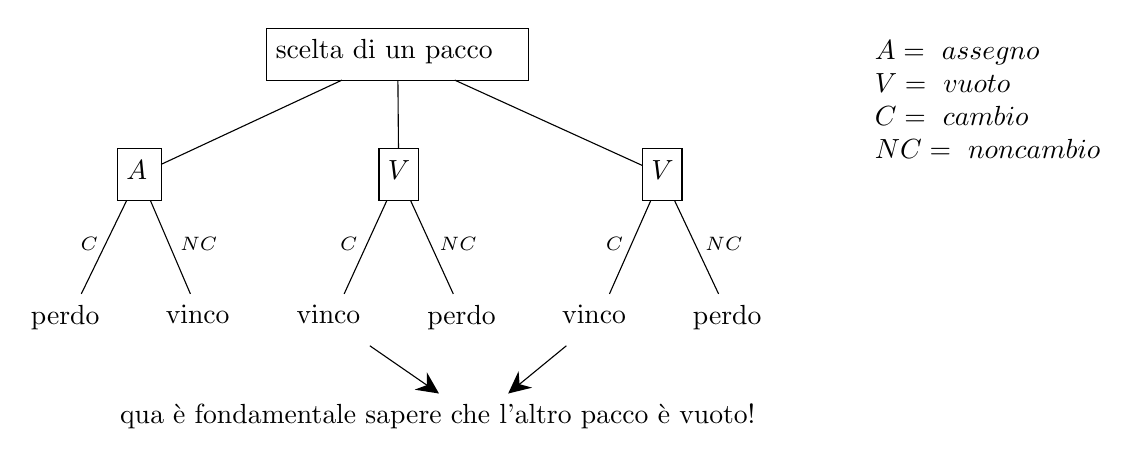
\begin{tikzpicture}[x=0.75pt,y=0.75pt,yscale=-1,xscale=1]
%uncomment if require: \path (0,230); %set diagram left start at 0, and has height of 230


% Text Node
\draw    (149,16) -- (275,16) -- (275,41) -- (149,41) -- cycle  ;
\draw (152,20) node [anchor=north west][inner sep=0.75pt]   [align=left] {scelta di un pacco};
% Text Node
\draw    (77,74) -- (98,74) -- (98,99) -- (77,99) -- cycle  ;
\draw (80,78.4) node [anchor=north west][inner sep=0.75pt]    {$A$};
% Text Node
\draw    (203,74) -- (222,74) -- (222,99) -- (203,99) -- cycle  ;
\draw (206,78.4) node [anchor=north west][inner sep=0.75pt]    {$V$};
% Text Node
\draw    (330,74) -- (349,74) -- (349,99) -- (330,99) -- cycle  ;
\draw (333,78.4) node [anchor=north west][inner sep=0.75pt]    {$V$};
% Text Node
\draw (34,148) node [anchor=north west][inner sep=0.75pt]   [align=left] {perdo};
% Text Node
\draw (99,148) node [anchor=north west][inner sep=0.75pt]   [align=left] {vinco};
% Text Node
\draw (162,148) node [anchor=north west][inner sep=0.75pt]   [align=left] {vinco};
% Text Node
\draw (225,148) node [anchor=north west][inner sep=0.75pt]   [align=left] {perdo};
% Text Node
\draw (290,148) node [anchor=north west][inner sep=0.75pt]   [align=left] {vinco};
% Text Node
\draw (353,148) node [anchor=north west][inner sep=0.75pt]   [align=left] {perdo};
% Text Node
\draw (77,196) node [anchor=north west][inner sep=0.75pt]   [align=left] {qua è fondamentale sapere che l'altro pacco è vuoto!};
% Text Node
\draw (434,18.4) node [anchor=north west][inner sep=0.75pt]    {$\begin{array}{l}
A=\ \text{assegno}\\
V=\ \text{vuoto}\\
C=\ \text{cambio}\\
NC=\ \text{non cambio}
\end{array}$};
% Text Node
\draw (58,115.4) node [anchor=north west][inner sep=0.75pt]  [font=\scriptsize]  {$C$};
% Text Node
\draw (106,115.4) node [anchor=north west][inner sep=0.75pt]  [font=\scriptsize]  {$NC$};
% Text Node
\draw (183,115.4) node [anchor=north west][inner sep=0.75pt]  [font=\scriptsize]  {$C$};
% Text Node
\draw (231,115.4) node [anchor=north west][inner sep=0.75pt]  [font=\scriptsize]  {$NC$};
% Text Node
\draw (311,115.4) node [anchor=north west][inner sep=0.75pt]  [font=\scriptsize]  {$C$};
% Text Node
\draw (359,115.4) node [anchor=north west][inner sep=0.75pt]  [font=\scriptsize]  {$NC$};
% Connection
\draw    (81.43,99) -- (59.57,144) ;
% Connection
\draw    (92.86,99) -- (112.14,144) ;
% Connection
\draw    (218.21,99) -- (238.79,144) ;
% Connection
\draw    (206.79,99) -- (186.21,144) ;
% Connection
\draw    (333.96,99) -- (314.04,144) ;
% Connection
\draw    (345.39,99) -- (366.61,144) ;
% Connection
\draw    (185.17,41) -- (98,81.61) ;
% Connection
\draw    (212.11,41) -- (212.39,74) ;
% Connection
\draw    (239.48,41) -- (330,82.18) ;
% Connection
\draw    (198.6,169) -- (229.43,190.3) ;
\draw [shift={(231.9,192)}, rotate = 214.63] [fill={rgb, 255:red, 0; green, 0; blue, 0 }  ][line width=0.08]  [draw opacity=0] (10.72,-5.15) -- (0,0) -- (10.72,5.15) -- (7.12,0) -- cycle    ;
% Connection
\draw    (293.27,169) -- (267.55,190.1) ;
\draw [shift={(265.23,192)}, rotate = 320.63] [fill={rgb, 255:red, 0; green, 0; blue, 0 }  ][line width=0.08]  [draw opacity=0] (10.72,-5.15) -- (0,0) -- (10.72,5.15) -- (7.12,0) -- cycle    ;

\end{tikzpicture}

Ad esempio, per rispondere terzo punto ci interessano solo gli eventi in cui ala seconda scelta cambio pacco (i rami sinistri). Vediamo che su $3$ possibili situazioni quelle in cui vinciamo sono $2$, i.e. $\PP(V_{\text{camb}}) =\frac{2}{3}$.

Analogamente, se non cambiamo (rami destri), su tre possibili situazioni quella vittoriosa è solo una, i.e. $\PP(V_{\text{cons}}) =\frac{1}{3}$.

\begin{oss}
	Intuitivamente: il conduttore aprendo un pacco ci sta dando delle informazioni in più: è come se, con la sua informazione, ci dicesse "il pacco rimasto (non il tuo) ha $\frac{2}{3}$ di probabilità di essere il pacco vincente". Cioè se prima avevo una probabilità di $\frac{2}{3}$ "distribuita su $2$ pacchi", adesso questa probabilità è tutta "concentrata sull'altro pacco". Quindi mi conviene cambiare pacco perché questo ha una probabilità più alta $\left(\frac{2}{3}\right)$ rispetto al mio $\left(\frac{1}{3}\right)$ di contenere l'assegno.


	% Pattern Info
	 
	\tikzset{
	pattern size/.store in=\mcSize, 
	pattern size = 5pt,
	pattern thickness/.store in=\mcThickness, 
	pattern thickness = 0.3pt,
	pattern radius/.store in=\mcRadius, 
	pattern radius = 1pt}
	\makeatletter
	\pgfutil@ifundefined{pgf@pattern@name@_v47zenp0g}{
	\pgfdeclarepatternformonly[\mcThickness,\mcSize]{_v47zenp0g}
	{\pgfqpoint{0pt}{-\mcThickness}}
	{\pgfpoint{\mcSize}{\mcSize}}
	{\pgfpoint{\mcSize}{\mcSize}}
	{
	\pgfsetcolor{\tikz@pattern@color}
	\pgfsetlinewidth{\mcThickness}
	\pgfpathmoveto{\pgfqpoint{0pt}{\mcSize}}
	\pgfpathlineto{\pgfpoint{\mcSize+\mcThickness}{-\mcThickness}}
	\pgfusepath{stroke}
	}}
	\makeatother
	\tikzset{every picture/.style={line width=0.75pt}} %set default line width to 0.75pt        

	\begin{tikzpicture}[x=0.75pt,y=0.75pt,yscale=-1,xscale=1]
	%uncomment if require: \path (0,260); %set diagram left start at 0, and has height of 260

	%Shape: Brace [id:dp5635373611818795] 
	\draw   (197.5,58) .. controls (197.5,62.67) and (199.83,65) .. (204.5,65) -- (224.5,65) .. controls (231.17,65) and (234.5,67.33) .. (234.5,72) .. controls (234.5,67.33) and (237.83,65) .. (244.5,65)(241.5,65) -- (264.5,65) .. controls (269.17,65) and (271.5,62.67) .. (271.5,58) ;
	%Shape: Brace [id:dp17280187716588213] 
	\draw   (197.5,188) .. controls (197.5,192.67) and (199.83,195) .. (204.5,195) -- (224.5,195) .. controls (231.17,195) and (234.5,197.33) .. (234.5,202) .. controls (234.5,197.33) and (237.83,195) .. (244.5,195)(241.5,195) -- (264.5,195) .. controls (269.17,195) and (271.5,192.67) .. (271.5,188) ;
	%Shape: Rectangle [id:dp09840376922489535] 
	\draw  [color={rgb, 255:red, 155; green, 155; blue, 155 }  ,draw opacity=1 ] (37.5,21) -- (280,21) -- (280,114.56) -- (37.5,114.56) -- cycle ;
	%Shape: Rectangle [id:dp5883671807012183] 
	\draw  [color={rgb, 255:red, 155; green, 155; blue, 155 }  ,draw opacity=1 ] (37.5,148) -- (280,148) -- (280,241.56) -- (37.5,241.56) -- cycle ;
	%Shape: Rectangle [id:dp7587181690994056] 
	\draw  [color={rgb, 255:red, 155; green, 155; blue, 155 }  ,draw opacity=1 ] (364.5,148) -- (462,148) -- (462,241.56) -- (364.5,241.56) -- cycle ;

	% Text Node
	\draw    (151,29) -- (170,29) -- (170,54) -- (151,54) -- cycle  ;
	\draw (154,33.4) node [anchor=north west][inner sep=0.75pt]    {$1$};
	% Text Node
	\draw    (201,29) -- (220,29) -- (220,54) -- (201,54) -- cycle  ;
	\draw (204,33.4) node [anchor=north west][inner sep=0.75pt]    {$2$};
	% Text Node
	\draw    (251,29) -- (270,29) -- (270,54) -- (251,54) -- cycle  ;
	\draw (254,33.4) node [anchor=north west][inner sep=0.75pt]    {$3$};
	% Text Node
	\draw (47,80) node [anchor=north west][inner sep=0.75pt]   [align=left] {probabilità};
	% Text Node
	\draw (154,76.4) node [anchor=north west][inner sep=0.75pt]    {$\frac{1}{3}$};
	% Text Node
	\draw (230,76.4) node [anchor=north west][inner sep=0.75pt]    {$\frac{2}{3}$};
	% Text Node
	\draw (185,123.4) node [anchor=north west][inner sep=0.75pt]    {$\Downarrow $};
	% Text Node
	\draw    (151,159) -- (170,159) -- (170,184) -- (151,184) -- cycle  ;
	\draw (154,163.4) node [anchor=north west][inner sep=0.75pt]    {$1$};
	% Text Node
	\draw    (201,159) -- (220,159) -- (220,184) -- (201,184) -- cycle  ;
	\draw (204,163.4) node [anchor=north west][inner sep=0.75pt]    {$2$};
	% Text Node
	\draw  [pattern=_v47zenp0g,pattern size=6pt,pattern thickness=0.75pt,pattern radius=0pt, pattern color={rgb, 255:red, 0; green, 0; blue, 0}]  (251,159) -- (270,159) -- (270,184) -- (251,184) -- cycle  ;
	\draw (254,163.4) node [anchor=north west][inner sep=0.75pt]    {$3$};
	% Text Node
	\draw (47,210) node [anchor=north west][inner sep=0.75pt]   [align=left] {probabilità};
	% Text Node
	\draw (154,206.4) node [anchor=north west][inner sep=0.75pt]    {$\frac{1}{3}$};
	% Text Node
	\draw (230,206.4) node [anchor=north west][inner sep=0.75pt]    {$\frac{2}{3}$};
	% Text Node
	\draw    (381,159) -- (400,159) -- (400,184) -- (381,184) -- cycle  ;
	\draw (384,163.4) node [anchor=north west][inner sep=0.75pt]    {$1$};
	% Text Node
	\draw    (431,159) -- (450,159) -- (450,184) -- (431,184) -- cycle  ;
	\draw (434,163.4) node [anchor=north west][inner sep=0.75pt]    {$2$};
	% Text Node
	\draw (384,206.4) node [anchor=north west][inner sep=0.75pt]    {$\frac{1}{3}$};
	% Text Node
	\draw (435,206.4) node [anchor=north west][inner sep=0.75pt]    {$\frac{2}{3}$};
	% Text Node
	\draw (312,189.4) node [anchor=north west][inner sep=0.75pt]    {$\iff $};


	\end{tikzpicture}
\end{oss}
\begin{enumerate}
	\item Consideriamo l'evento
	\begin{equation*}
		V_{\text{tc}} =\event{vinco giocando a testa o croce tra le due strategie}
	\end{equation*}
	Supponiamo la moneta equa e, senza perdita di generalità, assegnamo a $T$ la strategia di cambio pacco. Osserviamo che il lancio della moneta è indipendente dagli eventi $V_{\text{camb}}$ e $V_{\text{cons}}$. Usiamo ancora la formula delle probabilità totali, in questo caso con $\Omega =T\cup C$.
	\begin{align*}
		\PP(V_{\text{tc}}) & =\PP(V_{\text{tc}} \mid T)\PP(T) +\PP(V_{\text{tc}} \mid C)\PP(C) \\
		 & =\PP(V_{\text{camb}} \mid T)\PP(T) +\PP(V_{\text{cons}} \mid C)\PP(C) \\
		 & \indepeq \PP(V_{\text{camb}})\PP(T) +\PP(V_{\text{cons}})\PP(C) \\
		 & =\frac{2}{3} \cdotp \frac{1}{2} +\frac{1}{3} \cdotp \frac{1}{2} =\frac{1}{3} +\frac{1}{6} =\frac{1}{2}
	\end{align*}
	\item Introduciamo gli eventi
	\begin{align*}
		D&=\event{il conduttore apre il pacco di destra}\\
		P_{d} &=\event{il pacco di destra contiene il premio}\\
		P_{s} &=\event{il pacco di sinistra contiene il premio}
	\end{align*}
	Dal testo sappiamo che, poiché in tal caso il vincitore ha il pacco vincente,
	\begin{equation*}
		\boxed{\PP(D\mid A) =p}
	\end{equation*}
	$p$ è la probabilità che il conduttore apra il pacco di destra, sapendo che il vincitore ha il pacco vincente (cioè i due pacchi rimasti sono entrambi vuoti). Noi vogliamo calcolare
	\begin{equation*}
		\boxed{\PP(A\mid D) =?}
	\end{equation*}
	ovvero la probabilità che il pacco scelto inizialmente contenga il premio, sapendo che il conduttore ha aperto il pacco di destra. Per calcolarla usiamo la formula di Bayes.
	\begin{theorem}
		Sia $(\Omega,\Ac,\PP)$ uno spazio di probabilità. Siano $A\in \Ac$, $\{E_{k}\}_{k\in \NN} \subset \Ac$ una partizione discreta di $\Omega $. Se $\PP(A) ,\PP(E_{k})  >0,\forall k\in \NN$, allora
		\begin{equation*}
			\PP(E_{k} \mid A) =\frac{\PP(A\mid E_{k})\PP(E_{k})}{\sum_{k}\PP(A\mid E_{k})\PP(E_{k})}
		\end{equation*}
	\end{theorem}

	\begin{oss}
		La prima idea sarebbe stata quella di usare la formula di Bayes nella forma $\PP(A\mid D) =\frac{\PP(D\mid A)\PP(A)}{\PP(D)}$. Questa formula è però inutile nel nostro caso perché \textbf{non} sappiamo quanto vale $\PP(D)$. Utilizziamo quindi la formula sopra proposta.
	\end{oss}

	La partizione di $\Omega $ è data da $\{A,P_{d} ,P_{s}\}$, questi $3$ eventi ci dicono che pacco sta il premio. Allora
	\begin{align*}
		\PP(A\mid D) & =\frac{\overbrace{\PP(D\mid A)}^{p}\overbrace{\PP(A)}^{\frac{1}{3}}}{\underbrace{\PP(D\mid A)}_{p}\underbrace{\PP(A)}_{\frac{1}{3}} +\underbrace{\PP(D\mid P_{d})}_{0}\underbrace{\PP(P_{d})}_{\frac{1}{3}} +\underbrace{\PP(D\mid P_{s})}_{1}\underbrace{\PP(P_{s})}_{\frac{1}{3}}}\\
		 & =\frac{\frac{p}{3}}{\frac{p}{3} +\frac{1}{3}} =\frac{p}{p+1}
	\end{align*}

	\begin{oss}
		In questo caso l'informazione che abbiamo è una info \textit{storica}: dai dati che abbiamo raccolto abbiamo una informazione in più sul gioco e questa informazione \textit{non} dipende dalla scelta del conduttore. La probabilità $\PP$ si \textit{aggiorna} con questa nuova informazione (Teorema di Bayes).
	\end{oss}

	Analizziamo alcuni casi di valori di $p$
	\begin{enumerate}
		\item $\boxed{p=0}$ i.e. se il concorrente ha il pacco vincente, il pacco di destra non viene mai aperto. In altri termini, se il pacco di destra viene aperto, allora il concorrente non ha il pacco vincente. Questo è quello che ci dice il risultato trovato $\PP(A\mid D) =0$.
		\item $\boxed{p=1}$ i.e. se il concorrente ha il pacco vincente, allora certamente viene aperto il pacco di destra. Quindi, in tal caso, osservando l'apertura del pacco di destra siamo più propensi a credere che il concorrente abbia il premio $\PP(A\mid D) =\frac{1}{2}$.
		\item $\boxed{p=\frac{1}{2}}$ i.e. se il concorrente ha il pacco vincente, allora viene aperto indifferentemente uno dei due pacchi. Non abbiamo ulteriori informazioni, quindi non aggiorneremo le nostre ipotesi \textit{a priori}.
	\end{enumerate}
\end{enumerate}

\Soluzione

\Soluzione

\Soluzione

Introduciamo gli eventi
\begin{itemize}
	\item $R_{k} =$ \event{la $k$-esima pallina estratta è rossa}.
	\item $B_{k} =$ \event{la $k$-esima pallina estratta è bianca}.
\end{itemize}
Allora
\begin{enumerate}
	\item $\PP(R_{1}) =\frac{r}{r+b}$
	\item $\PP(R_{1} \cap B_{2}) =\PP(B_{2} \mid R_{1})\PP(R_{1}) =\frac{b}{r+b-1} \cdotp \frac{r}{r+b} =\frac{rb}{(r+b)(r+b-1)}$
	\item $
	\begin{aligned}
		\PP((B_{1} \cap R_{2}) \cup (R_{1} \cap B_{2})) & =\underbrace{\PP(B_{1} \cap R_{2})}_{\underbrace{\PP(R_{1} \mid B_{1})}_{\frac{r}{r+b-1}}\underbrace{\PP(B_{1})}_{\frac{b}{r+b}}} +\underbrace{\PP(R_{1} \cap B_{2})}_{\frac{rb}{(r+b)(r+b-1)}}\\
		 & \ \ \ \ \ \ \ \ \ \ \ \ \ \ \ \ -\underbrace{\PP((B_{1} \cap R_{2}) \cap (R_{1} \cap B_{2}))}_{0}\\
		 & =\frac{2rb}{(r+b-1)(r+b)}
	\end{aligned}$
	\item $
	\begin{aligned}
		\PP(R_{2}) & =\PP(R_{2} \mid B_{1})\PP(B_{1}) +\PP(R_{2} \mid R_{1})\PP(R_{1})\\
		 & =\frac{rb}{(r+b-1)(r+b)} +\frac{(r-1) b}{(r+b-1)(r+b)} =\frac{r}{b+r}
	\end{aligned}$
	\item $
	\begin{aligned}
		\PP(R_{3}) & =\PP(R_{3} \mid R_{1} \cap R_{2})\PP(R_{1} \cap R_{2}) +\\
		 & \ \ \ \ \ \ \ \ +\PP(R_{3} \mid B_{1} \cap B_{2})\PP(B_{1} \cap B_{2}) +\\
		 & \ \ \ \ \ \ \ \ +\PP(R_{3} \mid B_{1} \cap R_{2})\PP(B_{1} \cap R_{2}) +\\
		 & \ \ \ \ \ \ \ \ +\PP(R_{3} \mid R_{1} \cap B_{2})\PP(R_{1} \cap B_{2})
	\end{aligned}$
	Dove $\PP(R_{3} \mid R_{1} \cap R_{2})\PP(R_{1} \cap R_{2}) =\PP(R_{3} \mid R_{1} \cap R_{2})\PP(R_{2} \mid R_{1})\PP(R_{1})$ e così anche per gli altri pezzi. Si trova infine $\PP(R_{3}) =\frac{r}{b+r}$.
\end{enumerate}

\Soluzione

\Soluzione

\Soluzione

\Soluzione

\begin{enumerate}
	\item $\PP(B\mid A) =\frac{1}{5000} =0.0002\ =\ 0.02\%$
	\item $B\cap C=\emptyset $
	\item $A\indep C$
	\item $D=B\cup C$
	\item $\PP(B\mid A,D) =\frac{\PP(B,A,D)}{\PP(A,D)} =\frac{\PP(B,A)}{\PP(B,A) +\PP(C,A)} =\frac{1}{1+\frac{\PP(C,A)}{\PP(B,A)}} =\frac{1}{1+\frac{\PP(C\mid A)}{\PP(B\mid A)}} =\frac{1}{1+\frac{\PP(C)}{\PP(B\mid A)}}$
	\item Poiché $\PP(C) \leq \PP(D) =\frac{1}{100000}$, vale
	\begin{equation*}
	\PP(B\mid A,D) \geq \frac{1}{1+\frac{\PP(D)}{\PP(B\mid A)}} =\frac{1}{1+\frac{5}{100}} =\frac{20}{21} =0.9524=95.24\%
	\end{equation*}
	\item Sì è il caso che Ferrero continui ad indagare su Ambrogio.
\end{enumerate}

\Soluzione

Definiamo l'evento
\begin{equation*}
	B_{k} = \event{la $k$-esima pallina estratta è bianca}
\end{equation*}
Allora
\begin{enumerate}
	\item $\PP(B_{1}) =\frac{1}{2}$
	\item $\PP(B_{2} \mid B_{1}) =\frac{1}{2}$. Si rinforzano solo le rosse: dato che la prima estratta è bianca, alla seconda estrazione mi troverò ancora davanti un'urna con $1B$ e $1R$.
	\item Con la formula delle probabilità totali e ricordando $\Omega =B_{1} \cup B_{1}\complementary$ (alla prima deve essere estratta $B$ o $R$)
	\begin{equation*}
		\PP(B_{2}) =\underbrace{\PP(B_{2} \mid B_{1})}_{\frac{1}{2}}\underbrace{\PP(B_{1})}_{\frac{1}{2}} +\PP\left(B_{2} \mid B_{1}\complementary\right)\underbrace{\PP\left(B_{1}\complementary\right)}_{\frac{1}{2}}
	\end{equation*}

	Ora, $\PP\left(B_{2} \mid B_{1}\complementary\right) =\frac{1}{3}$, infatti se alla prima estrazione è uscita $R$, alla seconda estrazione nell'urna ci sono $2B$ e $1R$. Allora $\PP(B_{2}) =\frac{1}{4} +\frac{1}{6} =\frac{5}{12}$.

	\tikzset{every picture/.style={line width=0.75pt}} %set default line width to 0.75pt        

	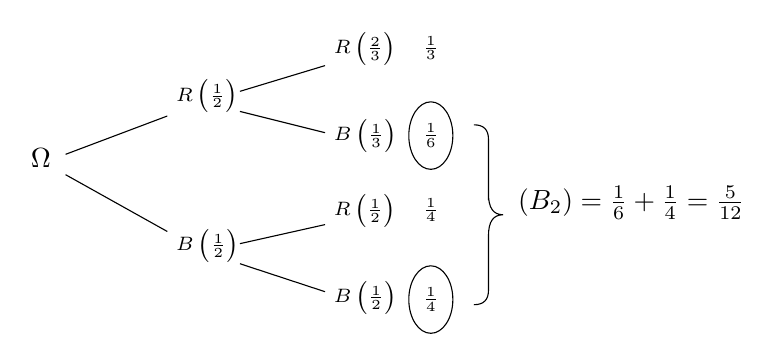
\begin{tikzpicture}[x=0.75pt,y=0.75pt,yscale=-1,xscale=1]
	%uncomment if require: \path (0,188); %set diagram left start at 0, and has height of 188

	%Shape: Brace [id:dp8335788707753122] 
	\draw   (292,157) .. controls (296.67,157) and (299,154.67) .. (299,150) -- (299,123.67) .. controls (299,117) and (301.33,113.67) .. (306,113.67) .. controls (301.33,113.67) and (299,110.34) .. (299,103.67)(299,106.67) -- (299,77.33) .. controls (299,72.66) and (296.67,70.33) .. (292,70.33) ;

	% Text Node
	\draw (77.25,80.4) node [anchor=north west][inner sep=0.75pt]    {$\Omega $};
	% Text Node
	\draw (147.25,47.4) node [anchor=north west][inner sep=0.75pt]  [font=\scriptsize]  {$R\left(\frac{1}{2}\right)$};
	% Text Node
	\draw (147.25,119.4) node [anchor=north west][inner sep=0.75pt]  [font=\scriptsize]  {$B\left(\frac{1}{2}\right)$};
	% Text Node
	\draw (223.25,24.4) node [anchor=north west][inner sep=0.75pt]  [font=\scriptsize]  {$R\left(\frac{2}{3}\right)$};
	% Text Node
	\draw (223.25,66.4) node [anchor=north west][inner sep=0.75pt]  [font=\scriptsize]  {$B\left(\frac{1}{3}\right)$};
	% Text Node
	\draw (223.25,102.4) node [anchor=north west][inner sep=0.75pt]  [font=\scriptsize]  {$R\left(\frac{1}{2}\right)$};
	% Text Node
	\draw (223.25,144.4) node [anchor=north west][inner sep=0.75pt]  [font=\scriptsize]  {$B\left(\frac{1}{2}\right)$};
	% Text Node
	\draw (271.22,33.52) node  [font=\scriptsize]  {$\frac{1}{3}$};
	% Text Node
	\draw    (271.22, 75.52) circle [x radius= 10.61, y radius= 16.26]   ;
	\draw (271.22,75.52) node  [font=\scriptsize]  {$\frac{1}{6}$};
	% Text Node
	\draw (271.22,111.52) node  [font=\scriptsize]  {$\frac{1}{4}$};
	% Text Node
	\draw    (271.22, 154.52) circle [x radius= 10.61, y radius= 16.26]   ;
	\draw (271.22,154.52) node  [font=\scriptsize]  {$\frac{1}{4}$};
	% Text Node
	\draw (312,98.73) node [anchor=north west][inner sep=0.75pt]    {$\PP(B_{2}) =\frac{1}{6} +\frac{1}{4} =\frac{5}{12}$};
	% Connection
	\draw    (179.25,54.2) -- (220.25,41.8) ;
	% Connection
	\draw    (179.25,63.88) -- (220.25,74.13) ;
	% Connection
	\draw    (95.25,84.55) -- (144.25,66.09) ;
	% Connection
	\draw    (95.25,94.36) -- (144.25,121.73) ;
	% Connection
	\draw    (179.25,127.59) -- (220.25,118.41) ;
	% Connection
	\draw    (179.25,137.26) -- (220.25,150.74) ;

	\end{tikzpicture}

	\item $\PP(B_{1} \cup B_{2}) =\underbrace{\PP(B_{1})}_{\frac{1}{2}} +\underbrace{\PP(B_{2})}_{\frac{5}{12}} -\underbrace{\PP(B_{1} \cap B_{2})}_{\frac{1}{4}} =\frac{6+5-3}{12} =\frac{2}{3}$

	$\PP(B_{1} \cap B_{2}) =\PP(B_{2} \mid B_{1})\PP(B_{1}) =\frac{1}{2} \cdotp \frac{1}{2} =\frac{1}{4}$

	Alternativamente:
	\begin{align*}
		\PP(B_{1} \cup B_{2}) & =1-\PP\left(B_{1}\comp \cap B_{2}\comp\right)\\
		 & =1-\PP\left(B_{2}\comp \mid B_{1}\comp\right)\PP\left(B_{1}\comp\right) =1-\frac{1}{3} =\frac{2}{3}
	\end{align*}
	\item $\PP(B_{1} \mid B_{2}) =\frac{\PP(B_{2} \mid B_{1})\PP(B_{1})}{\PP(B_{2})} =\frac{3}{5}$
	\item $
	\begin{aligned}
		\PP\left(\bigcap\limits_{k=1}^{n} B_{k}\right) & \overset{\text{Thm} \ 3.3\ JP}{=}\PP(B_{1})\PP(B_{2} \mid B_{1})\PP(B_{3} \mid B_{1} \cap B_{2}) \cdots \PP(B_{n} \mid B_{1} \cap \cdots \cap B_{n-1})\\
		 & =\left(\frac{1}{2}\right)^{n}
	\end{aligned}$
	
	Stiamo sfruttando il fatto che c'è rinforzo solo delle rosse e \textit{non} che abbiamo prove ripetute indipendenti!
	\item $
	\begin{aligned}
		\PP\left(\bigcap\limits_{k=1}^{n} B_{k}\complementary\right) & =\PP\left(B_{1}\complementary\right)\PP\left(B_{2}\complementary \mid B_{1}\complementary\right) \cdots \PP\left(B_{n}\complementary \mid B_{1}\complementary \cap \cdots \cap B_{n-1}\complementary\right)\\
		 & =\frac{1}{\cancel{2}} \cdotp \frac{\cancel{2}}{\cancel{3}} \cdots \frac{1}{n+1} =\frac{1}{n+1}
	\end{aligned}$

	Stiamo sfruttando il rinforzo delle rosse.
	\item $\underbrace{\PP\left(\bigcap\limits_{k=1}^{\infty } B_{k}\right) =\lim\limits_{n\rightarrow \infty }\PP\left(\bigcap\limits_{k=1}^{n} B_{k}\right)}_{\bigcap_{k=1}^{n} B_{k} \ \downarrow \ \bigcap_{k=1}^{\infty } B_{k}} =\liminf\limits_{n\rightarrow \infty }\left(\frac{1}{2}\right)^{n} =0$

	Abbiamo sfruttato la continuità dall'alto di $\PP$.
	\item $
	\begin{aligned}
		\PP\left(\left(\bigcap\limits_{k=1}^{\infty } B_{k}\right) \cup \left(\bigcap\limits_{k=1}^{\infty } B_{k}\complementary\right)\right) & =\underbrace{\PP\left(\bigcap\limits_{k=1}^{\infty } B_{k}\right)}_{0} +\PP\left(\bigcap\limits_{k=1}^{\infty } B_{k}\complementary\right) & \text{(unione disgiunta)}\\
		 & =\lim\limits_{n\rightarrow \infty }\PP\left(\bigcap\limits_{k=1}^{n} B_{k}\complementary\right) & \text{(continuità)}\\
		 & =\lim\limits_{n\rightarrow \infty }\frac{1}{n+1} =0 & 
	\end{aligned}$

\end{enumerate}

\Soluzione